\chapterimage{Collections.jpg} % Chapter heading image

\chapter{Collections}

The collection system resembles a tree that branches out from the treatment plant to collect the wastewater from individual sources.

\section{Wastewater Collection Piping}\index{Wastewater Collection Piping}	
	\begin{itemize}
		\item A \hl{lateral} is the piping that connects the public sewer to the building. 
		\item Laterals flow into larger lines called \hl{mains}.
		\item Mains carry the flow into the largest lines in the system, called \hl{trunk lines}. 
		\item A trunk line is the pipe that brings water into the treatment plant.
	\end{itemize}
\section{Sanitary Sewer Systems}\index{Sanitary Sewer Systems}

Sanitary sewer systems collect and convey wastewater from residential, commercial and industrial sources to a centralized wastewater treatment facility for treatment. 

\subsection{Storm-water systems}\index{Storm-water systems}

Storm-water systems are designed solely for the conveyance of storm-waters waters directly to streams, rivers, lakes, or the ocean.
 
\subsection{Combined sewer systems}\index{Combined sewer systems}
\begin{itemize}
\item Combined sewer systems collect and convey sanitary sewage and urban runoff in a common piping system.
\item Combined sewers could potentially cause serious water pollution problems during combined sewer overflow (CSO) events when wet weather flows exceed the sewage treatment plant capacity.
	\end{itemize}
\begin{center}
\includegraphics[scale=0.45]{SeperatedSystem1} \hspace{1 cm} \includegraphics[scale=0.45]{CombinedSystem1}
\end{center}
			\hspace{2.6cm} Separated System \hspace{3.2cm} \parbox{\textwidth}{Combined System}\\

\section{Collections Systems Basics}\index{Collections Systems Basics}
	\begin{itemize}
\item The primary type of a collection system is a \hl{gravity system}. A gravity system is so named because the wastewater flows down gradient in the sewer, driven by forces of gravity. 
\item The collection system includes the gravity sewers, force mains, manholes, pumping equipment, and other facilities that collect and convey the water to a wastewater treatment plant. 
\item Sewers are generally laid at a minimum slope to ensure open channel flow through the pipe at a \hl{minimum velocity of 2.0 feet per second}. The minimum velocity is required to ensure that solids do not settle out in the sewer.  
\item When the sewer lines reach a certain depth, the flow must be lifted back through a lift or pump station.  
\item \hl{Lift stations} are built whenever wastewater must be pumped to a higher altitude, whether it's to lift water up so that it can gravity flow or to pump it over a rise or hill.  
\item The discharge from the pump station may be to another gravity sewer at that location or through a pressurized force main. 
\item Key elements of lift stations include a wastewater receiving well (wet-well), pumps and piping with associated valves.
\item The size of the wet well affects the operating of the station. If a wet well is too small, excessive starting and stopping of the pump motors will occur, resulting in premature failure. If the wet well is too large, solids will tend to settle on the bottom, blocking the pump suction line and leading to the generation of hydrogen sulfide and methane.
\item The dry well is the portion of the dry well/wet well pumping station that houses the necessary equipment required to pump the wastewater. The dry well is so named because it is isolated from the incoming wastewater.
\item Centrifugal pumps are the most common type of pump found in wastewater pumping stations. 
\item In the USA, wastewater generated in a typical home is about 70 gal/day/person
\end{itemize}

\section{Collections Related Operational Issues}\index{Collections Related Operational Issues}
Infiltration and inflow (I/I) is the unwanted flow into the wastewater collections systems.
\subsection{Infiltration}\index{Infiltration}
\begin{itemize} 
\item Groundwater entering sanitary sewers through defective pipe joints and broken pipes is called infiltration. \hl{Remember:  \textbf{ground filters}}
\end{itemize}

\subsection{Inflow}\index{Inflow}
\begin{itemize} 
\item During rainstorms or snow thaws, large volumes of water may flow into the wastewater collections systems through leaky manhole covers or combined storm-water /wastewater connections.  In addition, private residences may have roof, cellar, yard, area, or foundation drains inappropriately connected to sanitary sewers.  These flows are termed as inflows. \hl{Remember: \textbf{rain flow}}
\end{itemize}

\textbf{Implications of I/I:}\\%$$$$$$$$$$$$$$$$$$$$%
\begin{itemize}
\item I/I decrease the efficiency and capacity of wastewater collection systems and treatment systems 
\item I/I can advance the need for capital costs to manage and treat flows
\item I/I contribute to the hydraulic overloading of treatment processes, which can affect public health and the compliance with NPDES permit requirements
\item I/I could cause Sanitary and combined sewer overflows(SSOs and CSOs) when wastewater flow volumes exceed the design capacity of the treatment plant 
\item I/I increase collection system and treatment facility operating costs
\end{itemize}

\subsection{Odors}\index{Odors}
\begin{itemize}
\item Hydrogen sulfide (H$_2$S), its associated compounds and methane are generated due to microbial

 activity in wastewater and the conveyance systems.  The \hl{rotten egg like smell} of hydrogen sulfide causes public nuisance odors, poses a health hazard for collections systems workers and causes corrosion of the system through its conversion to sulfuric acid.  The hydrogen sulfide generation is typically controlled by reducing the potential for septicity in wastewater through proper design of the system -  adequate velocities and adequate air space and through chemical treatment.
 \end{itemize}

\subsection{Fats, Oils and Grease (FOG)}\index{Fats, Oils and Grease (FOG)}
\begin{itemize}
\item FOG from food home, food establishments and industries affect the operation of the collection system
\item FOG has a tendency to accumulate in sewer pipes decreasing its wastewater carrying capacity.
\item Excessive FOG accumulation may cause sewer overflows
 \end{itemize}

\chapterimage{Preliminary.jpg} % Chapter heading image

\chapter{Preliminary Treatment}
% \begin{enumerate}[1.]
% 	\definecolor{shadecolor}{RGB}{200, 200, 240}

% 	%%%%%%%%%%%
% 	% LEVEL 2 %
% 	%%%%%%%%%%%

% 	\begin{snugshade*}
% 		\item \noindent\textsc{Wastewater Constituents}%$$$$$$$$$$$$$$$$$$$$%
% 	\end{snugshade*}
% 	Solids, organic matter, nutrients, pathogens and oil \& grease are the main target constituents of wastewater treatment operations.
% 	\begin{enumerate}[A.]%___________%
% 			\definecolor{shadecolor}{RGB}{225, 235, 235}

				%%%%%%%%%%%
				% LEVEL 3 %
				%%%%%%%%%%%
		% \begin{snugshade*}
		% 	\item \noindent\textsc{Organic Matter}%###############################%
		% \end{snugshade*}






			\begin{itemize}
				\item The objective of preliminary treatment is to remove coarse solids and other large materials often found in raw wastewater
				\item Removal of these materials is necessary to enhance the operation and maintenance of subsequent treatment units\\
				\item Preliminary treatment operations typically include a combination of the following processes:
					\begin{itemize}
						\item Screening
						\item Grinding or shredding
						\item Flow measurement
						\item Grit removal
						\item Pre-aeration
						\item Flow equalization
					\end{itemize}
			\end{itemize}

				
		\section{Process Elements of Preliminary Treatment}\index{Process Elements of Preliminary Treatment}	
			
		\subsection{Screening}\index{Screening}
					\begin{itemize}
						\item Screening is typically the first unit in a preliminary treatment
						\item Screening allows for the capture of coarse solids as pieces of cloths garbage so as to protect pumps and other units from clogging. 
						\item Screens may consist of vertical or inclined bars (bar racks or bar screens), wire mesh or perforated plates having either circular or rectangular openings. 
						\item Screens remove the large, entrained, suspended or floating solids such as pieces of wood, cloth, paper, plastics, garbage, etc.
						\item Debris collected on the screen can be cleaned manually or automatically using chain driven rakes 
						\item The retained material at screens - screenings, is collected and hauled to landfill for disposal
						\item The quantity of screenings removed varies by location and is a function of the clear opening of the screen.
						\item Barmuinitors combine the function of a screen and a grinder.  The ground material is returned to the wastewater flow for removal during primary treatment.
					\end{itemize}

\begin{figure}
\begin{center}
    \includegraphics[width=0.7\linewidth]{Barscreen}\\

Barscreen - No rakes
\end{center}
  \end{figure}
  
 \begin{center}
    \includegraphics[scale=0.6]{Blank}\\
\hspace{0cm} Video: Automatic Barscreen
  \end{center}
 
		\subsection{Grinding and Shredding}\index{Grinding and Shredding}

					\begin{itemize}
\begin{minipage}{\textwidth}	\item Comminutor(Grinder) consist of fixed, rotating or oscillating teeth or blades, acting together to reduce the solids to a size which will pass through fixed or rotating screens grind rags into small chunks
\item The comminutors are installed in wastewater channel and they grind the larger solids without actually removing them from the wastewater.  These devices may be installed before the screens or as a combination of screen and cutters (barmunitors).
					\end{minipage}	
					\end{itemize}
					\begin{minipage}{\textwidth}
					\begin{center}
      \includegraphics[width=0.3\linewidth, height=70mm]{Comminutor}\\
      Comminutor\\
\end{center}
    \end{minipage}

\begin{figure}[h]
    \includegraphics[width=\linewidth]{Comminutor1}\\
    \hspace{5cm}Schematic of comminutor placement in a channel\\
%    \caption{Comminutor Schematic}
  \end{figure}
  
		\subsection{Flow Measurement}\index{Flow Measurement}
					\begin{itemize}
						\item Wastewater flow to a treatment plant is not constant but varies in a diurnal (daily) pattern reflecting domestic water use activity.
						\item Continuous flow measurement is necessary in order to monitor diurnal variations in flow which may affect treatment plant efficiency.\\
						\item Devices used for flow measurement as part of the preliminary treatment can be placed in a channel or in a pipe.
					\end{itemize}

		\subsubsection{Devices for Flow Measurement in Channels}\index{Devices for Flow Measurement in Channels}

					\begin{itemize}
						\item Weirs: 
							\begin{itemize}
								\item Typically sharp crested weirs which are essentially metal plates installed perpendicular the flow.  The plate may a straight edge, a V-notch, or a trapezoidal opening.
								\item The weir plate in the channel causes an increase in the depth of the water behind the weir.  which is proportional to the flow rate.
								\item The flow rate can be determined by calculation or by reading the corresponding flow value to the depth of the water, from a chart specific for that weir. 
								
						
\begin{figure}[h!]
  \centering
  \begin{subfigure}[b]{0.4\linewidth}
    \includegraphics[width=\linewidth]{ChannelWeir}
    \caption{Weir in a channel}
  \end{subfigure}
  \hspace{1cm}
  \begin{subfigure}[b]{0.4\linewidth}
    \includegraphics[width=\linewidth]{WierTypes}
    \caption{Weir types}
  \end{subfigure}
\end{figure}
								
								
								
							\end{itemize}
						\item Parshall Flume:
							\begin{itemize}
								\item Parshall flume uses a narrow section in the channel as the restriction rather than the vertical plate of a weir.
								\item Like the weir, the restriction due to the narrow section of the flume, causes an increase in the depth of the water behind the weir (head) which is proportional to the flow rate.
								\item The flow rate can be determined by calculation or by reading the corresponding flow value to the depth of the water, from a chart specific for that Parshall Flume. 
								\end{itemize}

					\end{itemize}
\begin{figure}[h!]
  \centering
  \begin{subfigure}[b]{0.4\linewidth}
    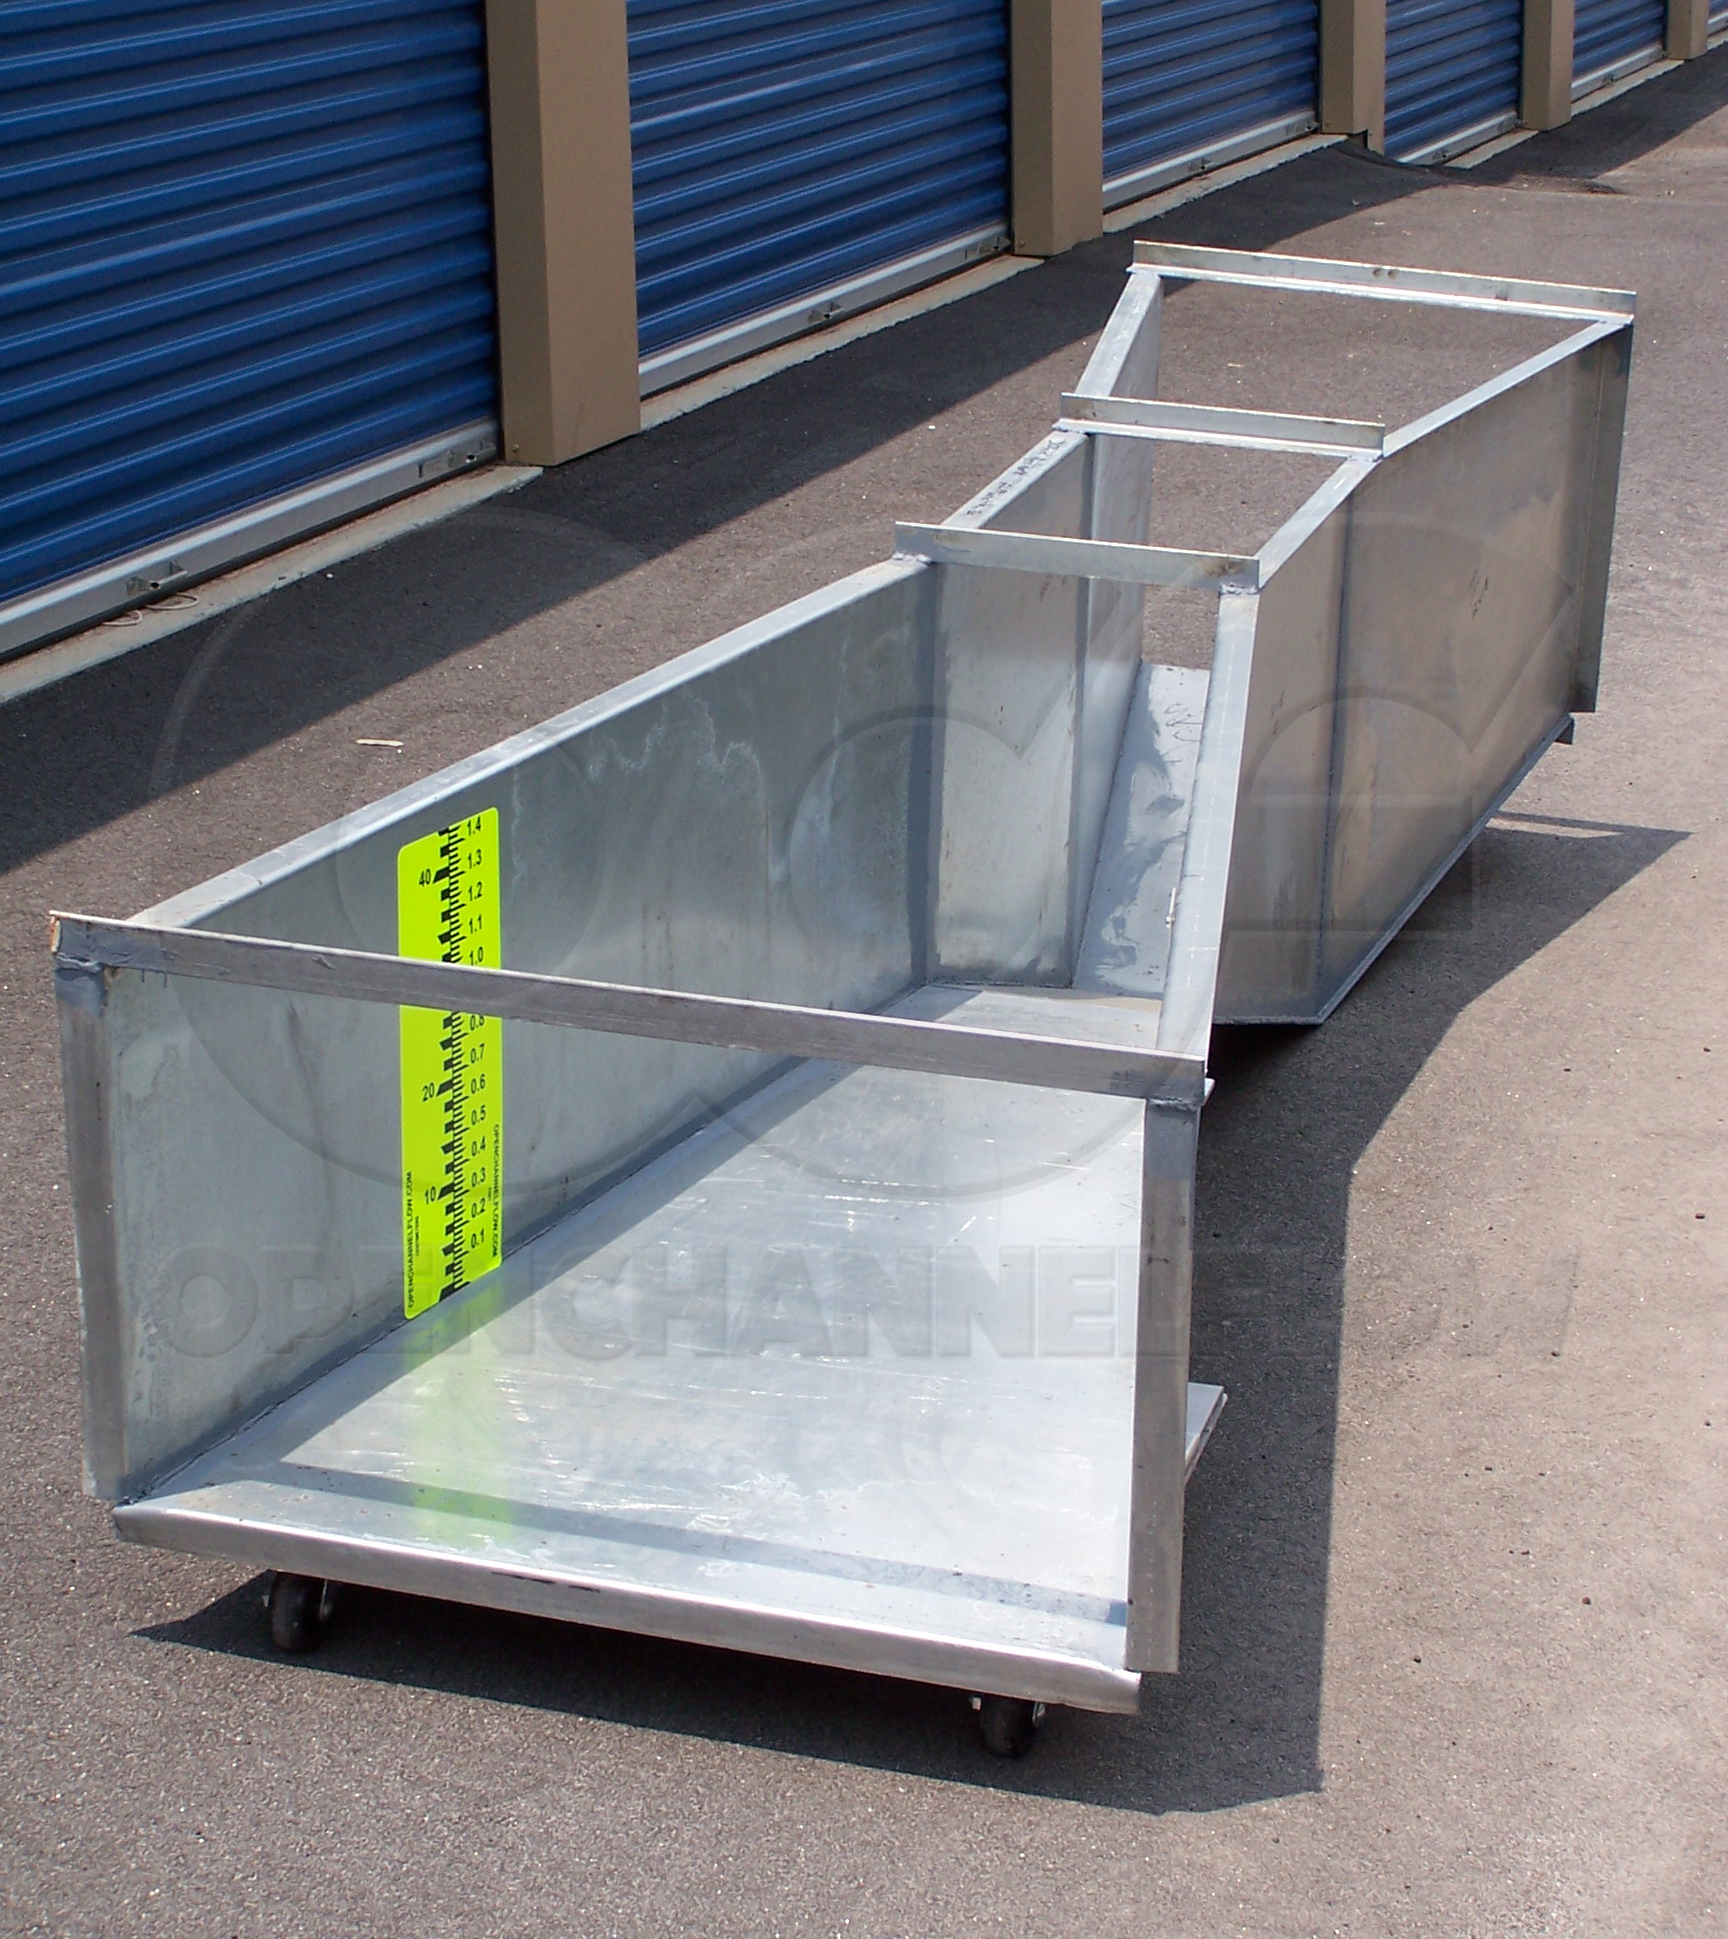
\includegraphics[width=0.75\linewidth]{parshallflume1}
    \caption{Parshall flume}
  \end{subfigure}
  \hspace{1cm}
  \begin{subfigure}[b]{0.4\linewidth}
    \includegraphics[width=\linewidth]{parshallflume2}
    \caption{Parshall flume with level sensor}
  \end{subfigure}
\end{figure}
		\subsubsection{Devices for Flow Measurement in Pipes}\index{Devices for Flow Measurement in Pipes}
					
					\begin{itemize}
						\item Venturi Tube:
							\begin{itemize}
								\item Measures the difference in pressure in the inlet and center section (throat)
								\item This pressure difference can then be mathematically converted to a flow rate.
								\item Works only when a pipe if flowing full
							\end{itemize}
						\item Magnetic Flow Meter (Magmeter):
							\begin{itemize}
								\item Magmeter is a pipe spool which has an electromagnetic coil surrounding it.  As the wastewater - a conducting material, flows through it, an electrical current is created proportional to the velocity of the conducting fluid (wastewater).
								\item Flow is automatically calculated by multiplying the velocity by the cross- sectional area of the pipe.
								\item Similar to the venturi meter, magmeter will read accurately only if the magmeter section of the pipe is flowing full and the wastewater is flowing through it at a certain minimum velocity.
							\end{itemize}
\begin{figure}[h!]
  \centering
  \begin{subfigure}[b]{0.4\linewidth}
    \includegraphics[width=0.9\linewidth]{magmeter1}
    \caption{Magmeter}
  \end{subfigure}
  \hspace{1cm}
  \begin{subfigure}[b]{0.45\linewidth}
    \includegraphics[width=\linewidth]{magmeter}
    \caption{Piping with magmeters}
  \end{subfigure}
\end{figure} 
					\end{itemize}
		\subsection{Grit Removal}\index{Grit Removal}
						\begin{itemize}
							\item Grit includes sand, gravel, cinder, eggshells, bone chips, seeds, coffee grounds, and large organic particles, such as food waste.
							\item Purpose of Grit removal:
								\begin{itemize} 
									\item to protect mechanical equipment from abrasion and abnormal wear 
									\item to reduce clogging caused by deposition of grit particles in pipes and channels, and 
				\item to prevent loading the treatment plant with inert matter that might interfere with the operation of treatment units such as anaerobic digester and aeration tanks.
			\end{itemize}
		\item Removal of organic material along with the grit is undesirable for two reasons:
			\begin{enumerate}
				\item It causes odor issues, and 
				\item Organic matter is a potential source of energy (digester gas)
			\end{enumerate}
		\item Grit Disposal: Grit removed is typically landfilled.
		\item Grit Volume:  The volume of grit collected measured in ft$^3$/MG.
		\item The rate of grit collection can range from 0.5 ft$^3$/MG to 30 ft$^3$/MG.
		\item Wastewater plants having a combined collection system must deal with much larger volumes of grit.
\end{itemize}
\subsubsection{Grit Removal Systems}\index{Grit Removal Systems}



			\begin{itemize}
			
					\item \noindent\textsc{Horizontal grit chambers:}

					\begin{itemize}
						\item These are rectangular channels 30 to 60 feet long and the water detention time is between 45 to 90 seconds
						\item Water passing through these channels is maintained at a relatively constant \hl{velocity of about 1 feet per second (fps)} which allows for the grit to settle while keeping the lighter organic material to stay in suspension and continue on into the primary clarifiers.
					\end{itemize}
	

						\item \noindent\textsc{Aerated grit chambers:}
	
					\begin{itemize}
						\item The 1 fps velocity is maintained by using aerators to create a rolling flow in the tank.
						\item Aeration is achieved using diffusers located on the bottom of one side of the grit chamber.
						\item Aerated grit chambers help create aerobic conditions in septic sewage. Aerobic conditions help improve the settleability of the sludge and increase both BOD and suspended solids removal in the primary clarifiers.
						\item Much larger and deeper than non-aerated units.
						\item The detention times are increased to 3 to 5 minutes.
					\end{itemize}

\begin{figure}[h!]
  \centering
  \begin{subfigure}[b]{0.46\linewidth}
    \includegraphics[width=0.8\linewidth]{HorizontalGritChamber}
    \caption{Horizontal grit chamber}
  \end{subfigure}
  \hspace{0.2cm}
  \begin{subfigure}[b]{0.5\linewidth}
    \includegraphics[width=0.8\linewidth]{AeratedGritChamber}
    \caption{Aerated grit chamber}
  \end{subfigure}
\end{figure} 					


						\item \noindent\textsc{Cyclonic/Vortex grit chamber:}


					\begin{itemize}
						\item The wastewater flows into a cylinder that tapers to a cone at one end.
						\item The flow whirls around the inside of the cylinder like a cyclone which causes the heavy grit to be slinged to the outside and it ultimately settles to the bottom from where it is withdrawn.
					\end{itemize}

\begin{figure}[h!]
  \centering
  \begin{subfigure}[b]{0.47\linewidth}
    \includegraphics[width=0.8\linewidth]{VortexGritChamber1}
    \caption{Vortex grit chamber design}
  \end{subfigure}
  \hspace{0.2cm}
  \begin{subfigure}[b]{0.43\linewidth}
    \includegraphics[width=0.8\linewidth]{VortexGritChamber}
    \caption{Vortex grit chamber installed}
  \end{subfigure}
\end{figure} 
	
\subsubsection{Grit Removal}\index{Grit Removal}		

		
			\begin{itemize}
				\item In the cyclonic/vortex grit chamber, the grit is scoured with water and is removed using pumps
				\item For the horizontal and aerated grit systems:
					\begin{itemize}
						\item Mechanical augers at the bottom of the grit chamber move the grit to one end of the tank where grit slurry pumps can pump it out of the tank to a grit separator.
						\item In some cases steep bottom slope is provided which will collect the grit at Central Point of Removal.
						\item Grit Removal is achieved by air pumps for small aerated grit chambers.
						\item Grit can also be removed by tubular conveyors, buckets type collectors, elevators screws conveyors, grit pumps and clam shell buckets
					\end{itemize}
			\end{itemize}
						\end{itemize}
%		\end{itemize}

\subsection{Flow Control}\index{Flow Control}	
	\begin{itemize} 
		\item Flow control is critical for grit removal, specifically for the horizontal and aerated grit chambers as excessive or inadequate velocities would lead to poor grit removal or cause excessive organic material settling along with the grit, respectively
		\item As the wastewater flows vary diurnally, it is important that velocity of the wastewater in the grit chamber should be maintained nearly constant - near 1 fps.
		
\begin{figure}[h]
    \includegraphics[width=\linewidth]{DiurnalFlow}\\
\begin{center}
Diurnal wastewater flow profile \\
\end{center}
%    \caption{Comminutor Schematic}
  \end{figure}		

		\item Constant velocity in a grit chamber is achieved by providing a \hl{proportional (Sutro) weir} at the outlet end of grit chamber.
		\item The shape of the opening between the plates of a proportional weir is made in such a way that the discharge is directly proportional to liquid depth in grit chamber resulting in maintaining a constant velocity of water even a the flow changes.
	\end{itemize}
\begin{figure}[h!]
  \centering
  \begin{subfigure}[b]{0.5\linewidth}
    \includegraphics[width=0.8\linewidth]{Sutroweir1}
    \caption{Proportional weir design}
  \end{subfigure}
  \hspace{1cm}
  \begin{subfigure}[b]{0.35\linewidth}
    \includegraphics[width=0.8\linewidth]{Sutroweir}
    \caption{Installed Proportional weir}
  \end{subfigure}
\end{figure} 

\subsection{Pre-aeration}\index{Pre-aeration}	
	\begin{itemize}
		\item Pre-aeration of the wastewater as part of the preliminary treatment may be provided as a separate process or increased detention time in an aerated grit chamber.
		\item Pre-aeration provides the follwoing benefits:
			\begin{itemize}
				\item freshens up wastewater by dissolving oxygen thereby reducing the wastewater septicity
				\item reduction of septicity allows for better settling - solids and BOD removal, in the following primary treatment process
				\item promotes grease separation which facilitates its removal during primary treatment
			\end{itemize}
	\end{itemize}
\subsection{Flow Equalization}\index{Flow Equalization}	

	\begin{itemize}
		\item Flow equalization involves storing a portion of peak flows for release during low-flow periods
		\item It prevents surges and allows for the operation of processes at design flows thus allowing for optimal physical, biological and chemical processes to take place.
		\item It results in saving capital costs as the processes may be built with a treatment capacity which is less than the peak flows
	\end{itemize}

\section{Preliminary Treatment Math Problems}\index{Preliminary Treatment Math Problems}

Preliminary Treatment math problems relate to the following:

\subsection{Channel Velocity and Flow Rate}\index{Channel Velocity and Flow Rate}
Flow Rate - Q (volume/time) = velocity (distance or length traveled /time) * surface area\\
Velocity is the speed at which the water is flowing.  It is measured in units of length/time – ft./sec.\\
Velocity of water flowing through can be calculated by dividing the flow rate by area of the flow stream.\\
\vspace{0.5cm}
$Velocity \enspace \dfrac{length}{time}= \dfrac{flow \enspace rate(\dfrac{volume \enspace or \enspace cubic \enspace length}{time})}{surface \enspace area \enspace in \enspace the \enspace direction \enspace of \enspace flow-square \enspace length}$\\
\vspace{0.5cm}
\textbf{For a flow in a channel:}\\
\vspace{0.5cm}
\hl{Example Problems:}\\
\begin{enumerate}[1.]
\item Calculate the velocity of a 14 MGD flow in a 6 ft wide channel with a water depth of two feet.\\
\begin{center}
\includegraphics[scale=0.5]{ChannelFlow3}
\end{center}
$Flow (Q) = Velocity (V) * Area (A)$\\
$\implies 14 \dfrac{MG}{day}* \dfrac{10^6 gal}{MG} * \dfrac{ft^3}{7.48 gal}*\dfrac{day}{24*60*60} = V \dfrac{ft}{sec}* 6 ft * 2 ft \implies 21.7 \dfrac{ft^3}{sec}= 12V\dfrac{ft^3}{sec}$\\
$\implies V \dfrac{ft}{sec}= \dfrac{21.7}{12}= \boxed{1.8\dfrac{ft}{sec}}$\\

\item Calculate the flow, in gpd, that would pass through a grit chamber 2 feet wide, at a depth of 6 inches, with a velocity of 1 ft /sec\\
Solution:\\
\includegraphics[scale=0.5]{ChannelFlow3}\\
$Q=V*A$\\
$Q=1\dfrac{ft}{s}*(2*0.5)ft^2=1\dfrac{ft^3}{s}$\\
$Q=1\dfrac{\cancel{ft^3}}{\cancel{s}}*\dfrac{(1440*60)\cancel{s}}{day}*7.48\dfrac{gal}{\cancel{ft^3}}=\boxed{646,272\dfrac{gal}{day}}$
\vspace{0.5cm}
\item A wastewater channel is 3.25 feet wide and is conveying a wastewater flow of 3.5 MGD. The wastewater flow is 8 inches deep. Calculate the velocity of this flow.\\
Solution:\\
\includegraphics[scale=0.5]{ChannelFlow3}\\
$Q=V*A \implies V=\dfrac{Q}{A}$\\
$\implies V\dfrac{ft}{s}=\dfrac{3.5\dfrac{\cancel{MG}}{\cancel{day}}*\dfrac{1000000\cancel{gal}}{\cancel{MG}}*\dfrac{ft^{\cancel{3}}}{7.48\cancel{gal}}*\dfrac{\cancel{day}}{(1440*60)s}}{(3.25*0.75)\cancel{ft^2}}=\boxed{2.2\dfrac{ft}{s}}$
\vspace{0.5cm}
\item A plastic float is dropped into a wastewater channel and is found to travel 10 feet in 4.2 seconds. The channel is 2.4 feet wide and is flowing 1.8 feet deep. Calculate the flow rate of this wastewater in cubic feet per second.\\
Solution:\\
$Q=V*A$\\
$\implies Q\Big(\dfrac{ft^3}{s}\Big)=\dfrac{10ft}{4.2s}*(2.4*1.8)ft^2=\boxed{10.3\dfrac{ft^3}{s}}$
\end{enumerate}

\subsection{Grit Removal Rates}\index{Grit Removal Rates}
\emph{Typical grit removal ranges from 0.5 to 30 ft$^3$/MG}\\
\vspace{0.3cm}
\hl{Example Problems:}\\
\begin{enumerate}[1.]
\item At a wastewater treatment plant which receives a flow rate of 650,000 gallons per day, a total of 50 cubic feet of grit was removed for the month. Calculate the rate of grit removal assuming 30 days in a month.\\
Solution:\\
$Grit Removal\dfrac{ft^3}{MG}=50\dfrac{ft^3}{ \cancel{month}}*\dfrac{\cancel{month}}{30\cancel{days}}*\dfrac{\cancel{day}}{650,000\cancel{gal}}*1,000,000\dfrac{\cancel{gal}}{MG}=\boxed{2.6\dfrac{ft^3}{MG}}$
\end{enumerate}

\chapterimage{Week3Clarifier1.jpg} % Chapter heading image

\chapter{Primary Treatment}

%\section{Background}\index{Background}
\begin{itemize}
\item Synonyms:  primary treatment basin, primary clarifier, sedimentation basin, primaries, clarifier

	
		\item Primary treatment is after preliminary treatment and 				before secondary treatment
		\item Its two main objectives are: 
			\begin{itemize}
				\item Remove settleable solids
				\item Remove floatable solids
			\end{itemize}
		\item This is a physical process which relies on the physical 			properties - how heavy or light the suspended solids particles 		are to effect its separation
		\item Provides quiescent conditions for the influent 					wastewater for the heavier solids to settle and the lighter 			solids to float
		\item Removes settleable solids and floatables
		\item Settled solids are removed as sludge from the bottom of 			the clarifier
		\item Floatable solids including oil and grease are also 				removed, as scum from the surface\\
		\item The shape of the primary clarifier is either rectangular 		or circular
	
		\item Effective solids removal in the primary clarifiers will 			reduce the loading on the expensive secondary treatment 				process.
		\item The amount of solids removed during primary treatment 			may be enhanced by chemical addition - ferric or ferrous 				chloride as a coagulant and anionic polymer as the flocculant.  		This is called Chemically Enhanced Primary Treatment (CEPT).

			\begin{center}
				\includegraphics[scale=0.9]{RectangularClarifier}\\
				Cross section of a Rectangular Clarifier\\

				\includegraphics[scale=0.1]{Blank}\\
				\includegraphics[scale=0.6]{CircularClarifierAI}\\
				Schematic cross section of a circular clarifier\\
				\includegraphics[scale=0.1]{Blank}\\
				\includegraphics[scale=0.5]{CircularClarifier3}\\
				Cross section of a circular clarifier\\
			\end{center}
				\includegraphics[scale=0.03]{Blank}\\
\item \textbf{Typical Removal Rates:}\\
\begin{itemize}
\item \hspace{10mm} BOD removal – 25\% to 40\% and about 60\% with CEPT
\item \hspace{10mm} Suspended solids (SS) removal – 40\% to 60\% and about 75\% with CEPT
\item \hspace{10mm} Settleable Solids removal - $>$90\%
\end{itemize}
\end{itemize}

\section{Clarifier Zones}\index{Clarifier Zones}
				
\subsection{Inlet Zone}\index{Inlet Zone}		
				\begin{itemize}
					\item Inlet Zone is where the water enters the end 					of a rectangular tank, or the center of a circular 					or square tank.
					\item The Inlet Zone is designed to accomplish two 					objectives:
						\begin{enumerate}
							\item Reduce the velocity (dissipate 									energy in the incoming water)
							\item Distribute the flow evenly
						\end{enumerate}
					\item The inlet zone is equipped with a baffle.  					Inlet baffle reduces the velocity of the 							influent flow, prevent short circuiting which 							could cause solids being carried over to secondary 					treatment.  
						\begin{itemize}
							\item Circular tanks are equipped with a 								collar-type circular baffle that directs 								the water down as it enters the center of 								the tank.
							\item Rectangular tanks will have a plate 								baffle in front of the opening for the 									wastewater flow into the clarifier and 									another baffle just upstream - a 										perforated wall or a picket fence type 									baffle that spreads the water laterally 								across the inlet end of the tank.\\


\begin{figure}[h!]
  \centering
  \begin{subfigure}[b]{0.4\linewidth}
    \includegraphics[width=0.8\linewidth]{InfluentBaffle}
    \caption{Rectangular clarifier influent baffle}
  \end{subfigure}
  \hspace{1cm}
  \begin{subfigure}[b]{0.4\linewidth}
    \includegraphics[width=\linewidth]{CircularClarifierInfluentBaffle}
    \caption{Circular clarifier influent baffle}
  \end{subfigure}
\end{figure}	
	
%							\begin{center}
%							\includegraphics[scale=0.65]												{InfluentBaffle}\\
%							Rectangular clarifier influent baffle
%							\end{center}
%							
%														\begin{center}
%							\includegraphics[scale=0.65]												{CircularClarifierInfluentBaffle}\\
%							Circular clarifier influent baffle
%							\end{center}	
						\end{itemize}
				\end{itemize}

\subsection{Settling Zone}\index{Settling Zone}
			\begin{itemize}
				\item This is the largest portion of the tank where 					solids settle.
				\item The water velocity is reduced to 0.03-0.05 fps 					and the detention time is about 1.5 to 2 hours. 
				\item A clarifier is said to be short circuiting if 					the velocity of the water is greater in some sections 					than in others. The water passing through the higher 					velocity region will have a reduced detention time and 				settleable solids will carry through with this water 					as it goes over the weir.  Short circuiting is 							prevented by appropriately designing inlet baffles and weir plates (at the Outlet Zone).
			\end{itemize}

\subsection{Sludge Zone}\index{Sludge Zone}
			\begin{itemize} 
				\item Sludge zone is the bottom of the tank where the 					settled sludge collects and compacts.
				\item Sludge blanket depth should be measured and 						sludge should be removed at least every shift. A 						desirable blanket depth is typically established and 					the sludge pumping rate and regimen is established to 					maintain that desired sludge blanket level.
				\item Sludge rakes push the sludge to one end or the 					center of the tank so that it can be pumped out. 
				\item The rake drive is usually equipped with a torque 				indicator. A shear pin in the drive shaft will break 					to prevent damage to the gearbox or drive shaft. 
				\item Failure to remove sludge often enough will 						result in the sludge becoming septic releasing gas 						bubbles which hinders the sludge settling and also 						result in causing odor problems.
				\item The sludge from the primary clarifiers needs to 					be stabilized prior to its disposal.  The sludge 						(solids) from the primary clarifiers are mixed with 					the solids from the secondary treatment process and 					stabilized typically using a sludge digestion process. 
			\end{itemize}
\subsection{Skimming Zone}\index{Skimming Zone}

			\begin{itemize}
				\item The skimming zone is at the surface of the tank 					for scum removal
				\item Lighter solids and greases float to the surface 					of the clarifier as scum
				\item In Circular Clarifiers:  Floating matter is 						skimmed by a skimmer arm that is supported by the 						sludge rake and rotates with it around the tank. The 					floating matter is pushed over the beach plate by the 					wipers attached to the skimmer arm and into a scum box 				attached to the tank wall.\\
				\item In Rectangular Clarifiers:  The flights act as 							skimmers when the chain brings them to the surface and 				pushes the scum towards the scum troughs.  The scum 					trough may be designed to rotate (tip) periodically 					for the scum to flow in from the water surface.\\
							
				\item The scum collected from the primary clarifiers is sent 				to the digester for treatment along with the sludge 					removed.\\ 

				\vspace{1cm}
									\begin{center}
					\includegraphics[scale=0.06]{RotatingScumTrough}\\
					Rectangular clarifier scum trough\\
									\includegraphics[scale=0.02]{Blank}\\
				\end{center}	

				\item The flights in the rectangular clarifier are supported 				at the top by two parallel rails running along the 						length of the clarifier.\\
				\item There are wear plates (strips) installed at the 						clarifer bottom and on top of the rails to prevent the 				flights from riding directly on those surfaces.  To 					reduce friction, the flights have a wearing shoe 						attached.  
				\item Both the wear strip and the wearing shoe 					are disposable items and are replaced at fixed 							intervals.\\			
				\begin{center}
					\includegraphics[scale=0.07]												{RectangularClarifierComponents}\\
					Rectangular clarifier flights\\
				\end{center}						  
\end{itemize}

\subsection{Outlet Zone}\index{Outlet Zone}
			\begin{itemize}
				\item  This is the part of the clarifier where the 						settled water leaves to go to the secondary treatment 					processes.
				\item A channel called the effluent launder collects 					the effluent flow and directs it to the primary 						effluent piping. 
				\item Weirs are installed along the edge of the effluent launder channel to skim the water evenly off the surface of the tank. The most common type of effluent weir is a V-notch (or saw-tooth) weir.   A V-	notch weir is a plate that has notches, about 2-3 						inches deep, cut in it every 6-8 inches. If the weir is clean and level, it will remove water evenly all 					the way around the edge of the tank. This minimizes 					the upward velocities near the effluent launder and 					improves removal efficiencies. If the weir plate is not level or part of the weir becomes clogged with 				slime or debris, short-circuiting will result because 					more water will pass over the low side or the clean notches of the weir. Short-circuiting will cause poor 					settling and uneven sludge blanket buildup.
				\item In rectangular tanks the water leaves at the end 	opposite the influent.
												  
				\item In circular  tanks the water leaves at the edge of the tank.
				\item Also, in the circular clarifiers, an effluent baffle, just upstream of the weir, 					is installed to prevent floating solids from going 						over the weir.
				\begin{center}
					\includegraphics[scale=0.04]												{CircularClarifierComponents1}\\
					Circular clarifier skimmer arm, effluent baffle and v-notch weir\\
				\end{center}
				
			\vspace{0.8cm}
					\begin{center}
					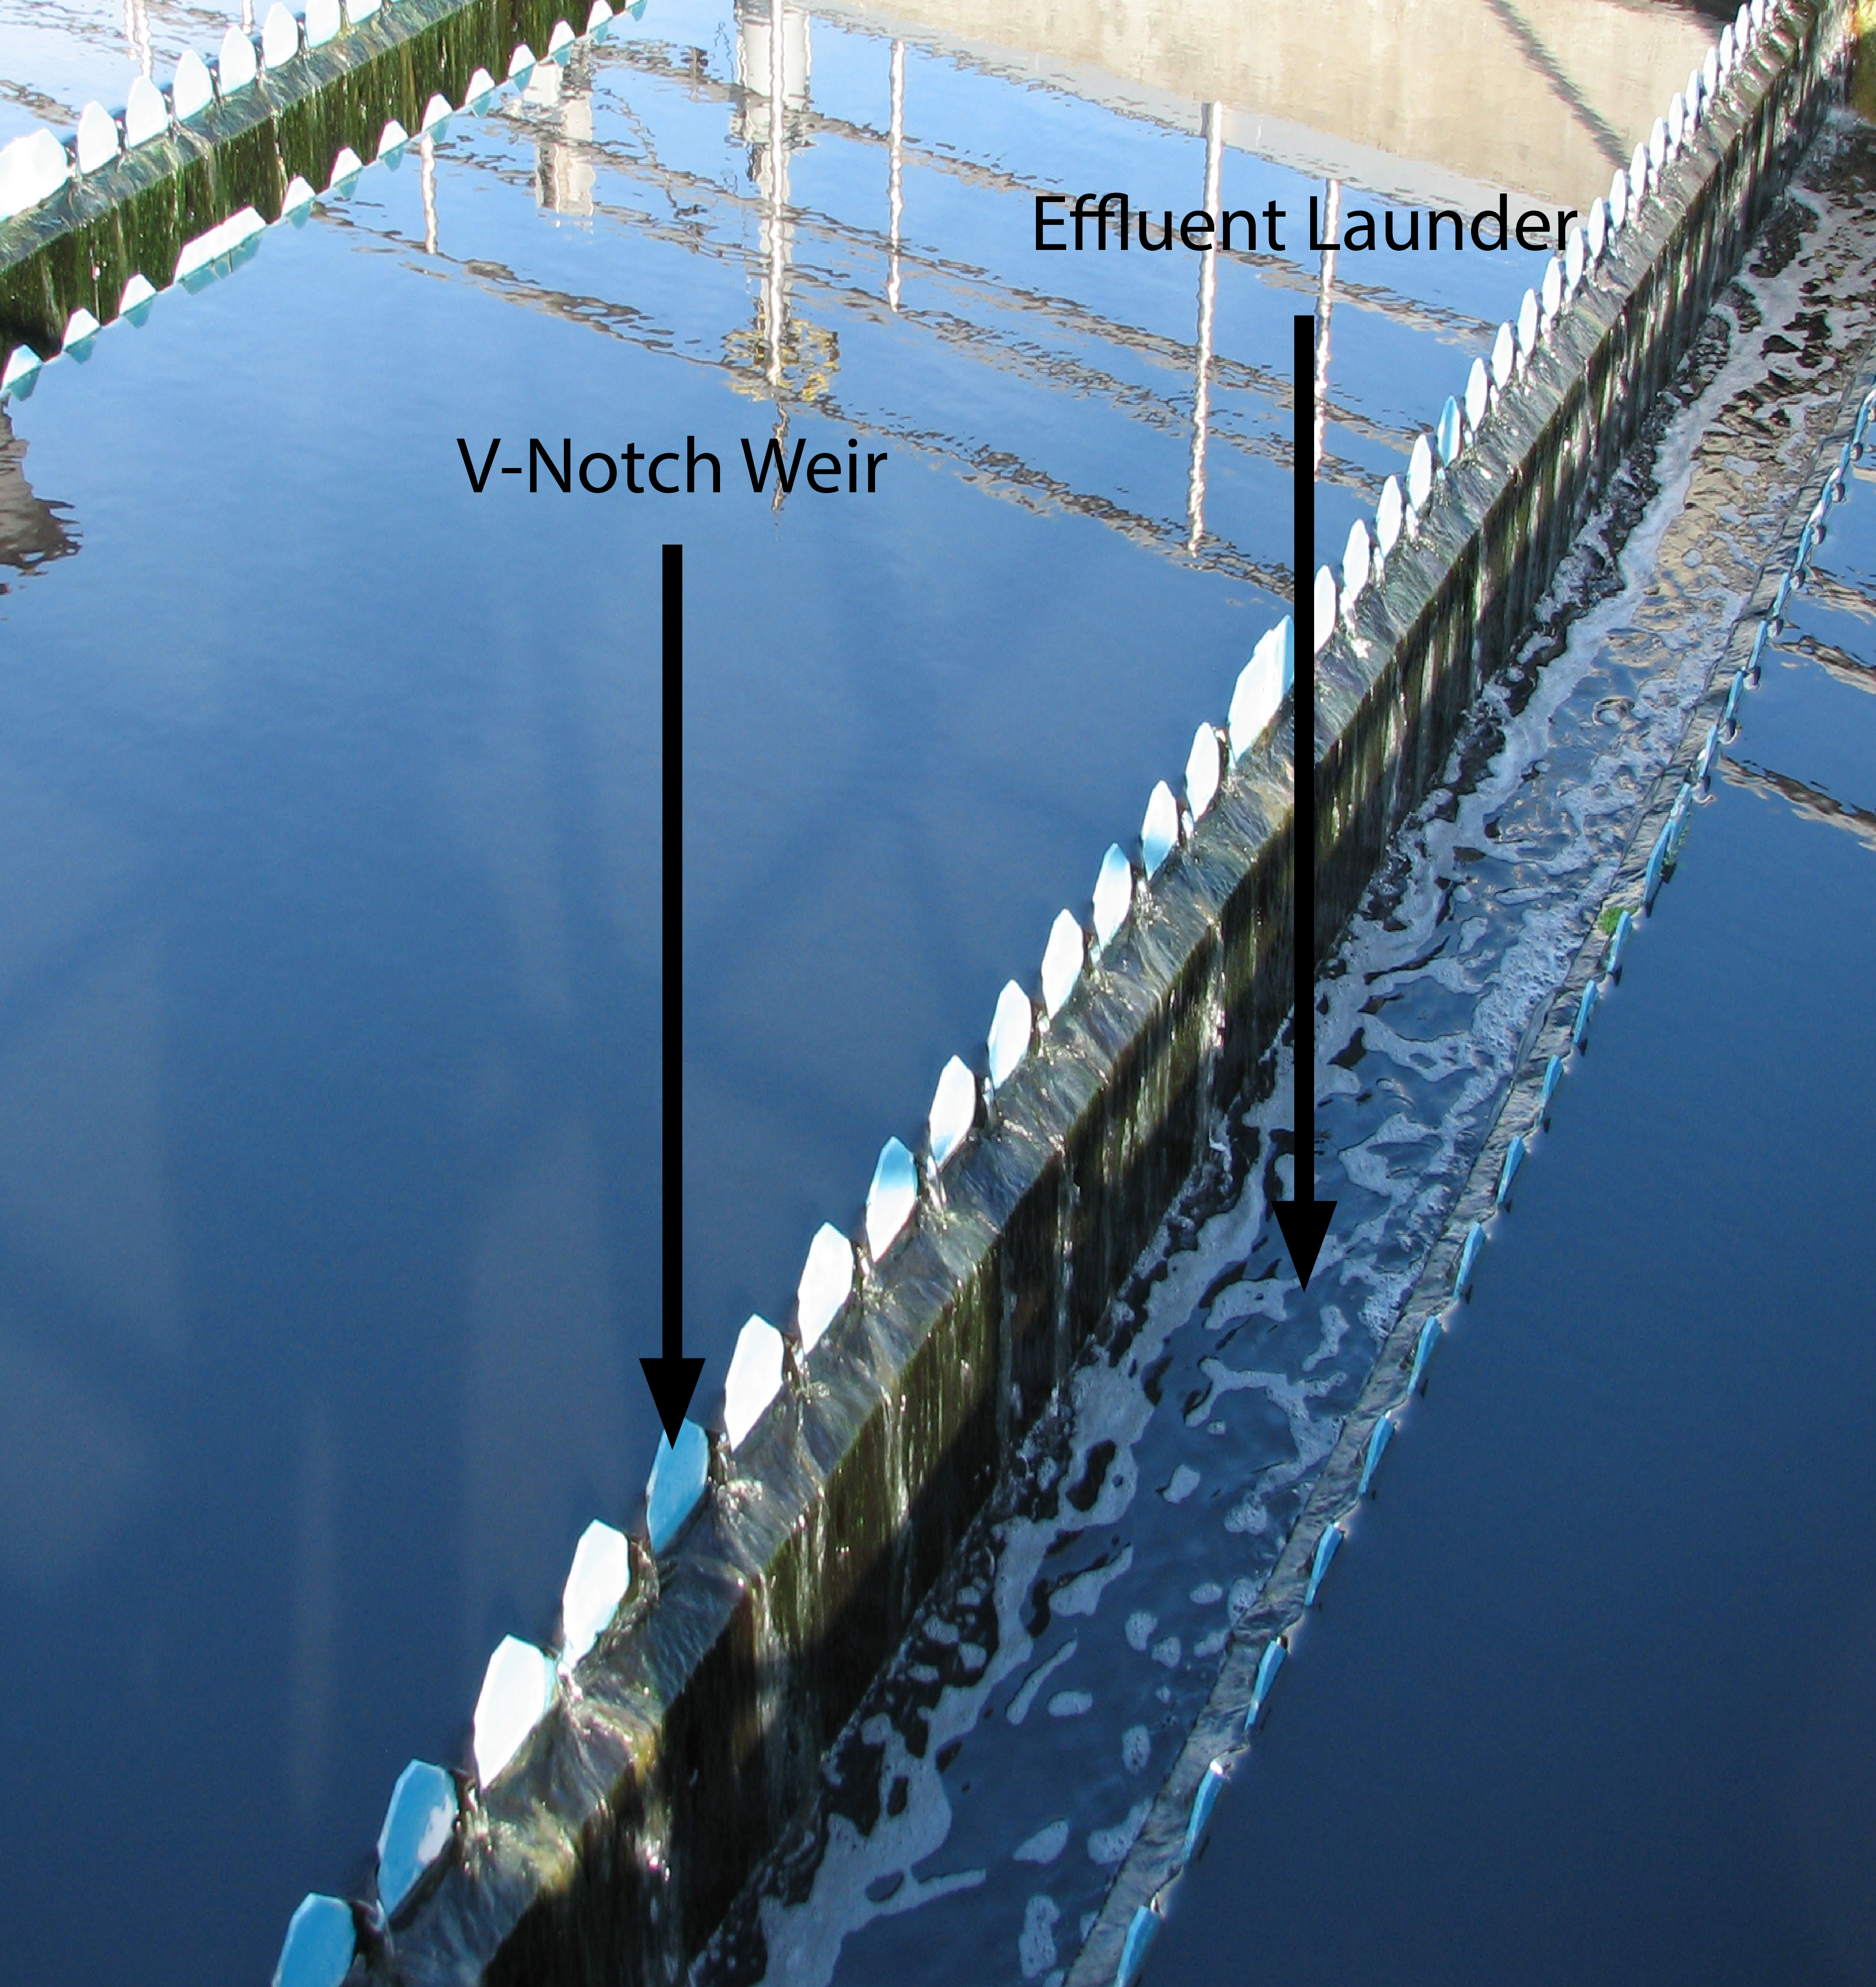
\includegraphics[scale=0.07]												{RectangularClarifierWeir}\\
					Rectangular clarifier v-notch weir and launder\\
				\end{center}			
												  
			\end{itemize}


\section{Sludge Pumping}\index{Sludge Pumping}

	\begin{itemize}
		\item The sludge pumping from the clarifier must be adequate 			to prevent sludge from going septic. Septic sludges are much 			more difficult to thicken or de-water and cause odor issues. 
		\item Primary sludge normally averages 4-6\% solids. 
		Generally positive displacement pumps are used for primary 				sludge
		\item The pumping cycles must be designed to provide the 				thickest sludge possible.
		\item Excessive pumping or pumping without building solids to 			build up leads to pumping thinner (more water) sludge.
	\end{itemize}
\section{Design Parameters}\index{Design Parameters}
	\begin{itemize}
	\setlength\itemsep{1em}
		\item \textbf{Clarifier depth} – 8 to 12 feet
		\item \textbf{Hydraulic or surface loading}
			\begin{itemize}
			\item This rate is important to ensure good settleable 					solids removal efficiency
			\item It is expressed in terms of gallons per day per 					square foot (gpd/sq ft) of tank surface area
			\item Typical surface loading rate used for the design of 				primary clarifiers range between 300 to 1,400 gpd/sq ft, 				depending on the nature of the solids and the treatment 				requirements. Lower loading rates are frequently used in 				small plants in cold climates. In warm regions, low rates 				may cause excessive detention which could lead to 						septicity.
			\end{itemize}
	\end{itemize}
\section{Math Problems}\index{Math Problems}

Types of Math Problems Related to Primary Sedimentation 

%\item Finding the clarifier hydraulic or surface loading rate
%\item Finding the clarifier detention time
%\item Finding the clarifier weir overflow rate
%\item Finding the clarifier removal efficiency
%\item Solids removal calculations
%\end{enumerate}
%\begin{enumerate}

\subsection{Hydraulic or Surface Loading Rate}\index{Hydraulic or Surface Loading Rate}

The hydraulic or surface loading rate measures how rapidly wastewater moves through the primary clarifier.  It is measured in terms of the number of gallons flowing each day through one square foot surface area of the clarifier. 
$$Clarifier \enspace hydraulic \enspace loading \enspace 	\Big(\dfrac{gpd}{ft^2}\Big) =\dfrac{Clarifier \enspace influent 	\enspace flow (gpd)}{Clarifier \enspace surface \enspace area 	(ft^2)}$$ 
		Rectangular clarifier surface area  = width * length\\
		Circular clarifier surface area  = 0.785 * Diameter$^2 $\\
\subsection{Detention Time}\index{Detention Time}

Detention time is the length of time that wastewater stays in the settling tank is called the detention time.  It is also the time it takes for a unit volume of wastewater to pass entirely through a primary clarifier\\
$$Clarifier \enspace detention \enspace time \enspace (hr) = 	\dfrac{ Clarifier \enspace volume (cu.ft \enspace or \enspace gal)}{Influent \enspace flow \enspace (cu.ft \enspace or \enspace gal)/hr)}$$
Rectangular clarifier volume = width * length * depth of water\\
Circular clarifier volume = 0.785 * Diameter$^2$ * depth of water\\
Typically volume is calculated in cu. ft and influent flow is given in gallons.  Use 7.48 gal/ft$^3$ conversion factor to convert volume in cu. ft to gallons.\\

\subsection{Weir Overflow Rate}\index{Weir Overflow Rate}
The weirs at the end of the primary clarifier allow for the even distribution of the the outlet flow across the entire length of the weir.  An adequate length of weir is needed to ensure smooth and even flow of wastewater over the weirs.  Weir overflow rate measures the number of gallons of wastewater per day flowing over one foot of weir. 

		$$Weir \enspace over \enspace flow \enspace rate \Big(\dfrac{gpd}{ft}\Big) =\Big(\dfrac{Clarifier \enspace influent \enspace  flow (gpd)}{Total \enspace effluent 					\enspace weir \enspace length \enspace (ft)}\Big)$$
		Circular clarifier weir length = 3.14 * Diameter\\

\hl{Example problem for (a), (b) and (c) above:}\\
		\vspace{0.2cm}
A circular clarifier receives a flow of 11 MGD.  If the clarifier is 90 ft. in diameter and is 12 ft. deep, what is: a) the hydraulic/surface loading rate, b) clarifier detention time in hours, and c) weir overflow rate?\\
		\vspace{0.2cm}
a) Hydraulic/surface loading rate:\\
$Clarifier \enspace hydraulic \enspace loading \enspace 	\Big(\dfrac{gpd}{ft^2}\Big) ==\dfrac{\dfrac{11\cancel{MG}}{{day}}*\dfrac{10^6gal}{\cancel{MG}}}{0.785*90^2 ft^2}=\boxed{1,730gpd/ft^2}$\\
		\vspace{0.5cm}
b) Clarifier detention time:\\
$Clarifier \enspace detention \enspace time \enspace (hr) = 	\dfrac{ Clarifier \enspace volume (cu.ft \enspace or \enspace gal)}{Influent \enspace flow \enspace (cu.ft \enspace or \enspace gal)/hr)}$\\
		\vspace{0.2cm}
$Clarifier \enspace detention \enspace time \enspace (hr) = 	\dfrac{(0.785*90^2*12)\cancel{ft^3}}{\dfrac{11\cancel{MG}}{\cancel{day}}*\dfrac{10^6\cancel{gal}}{\cancel{MG}}*\dfrac{\cancel{ft^3}}{7.48\cancel{gal}}*\dfrac{\cancel{day}}{24hrs}}=\boxed{1.2hrs}$\\
		\vspace{0.5cm}
c) Weir overflow rate:\\
		\vspace{0.2cm} 
$Weir \enspace overflow \enspace rate \Big(\dfrac{gpd}{ft}\Big) =\dfrac{\dfrac{11\cancel{MG}}{{day}}*\dfrac{10^6gal}{\cancel{MG}}}{3.14*90 ft}=\boxed{38,924gpd/ft}$\\

\subsection{Removal Efficiency}\index{Removal Efficiency}		
Primary sedimentation removes suspended wastewater solids which includes BOD.  The efficiency of the primary is established as the percentage of the amount of parameter removed.  The parameter may quantified as mass (lbs) or as concentration (mg/l).

$$Removal \enspace efficiency (\%) = \dfrac{Parameter  \enspace In - Parameter  \enspace Out}{Parameter \enspace In} * 100$$

For TSS removal:\\
$$TSS \enspace Removal \enspace efficiency (\%) = \dfrac{TSS  _{In} \enspace(mg/l)  - TSS_{Out} \enspace(mg/l)  }{TSS _{In} \enspace(mg/l)  } * 100$$

For BOD removal:\\
$$BOD \enspace Removal \enspace efficiency (\%) = \dfrac{BOD_{In} \enspace(mg/l)  - BOD_{Out} \enspace(mg/l)  }{BOD _{In} \enspace(mg/l)  } * 100$$
\subsection{Solids Removal}\index{Solids Removal}	

\hl{\textbf{Type 1 Problems:}  These involve calculating lbs of solids removed given any two of the following TSS parameters - inlet concentration, outlet concentration and removal efficiency.}\\
a. If the inlet and outlet concentrations are given, calculate the mg/l of TSS removed using: 
$$TSS_{removed} = TSS_{in}(mg/l) - TSS_{out} (mg/l) $$
Then knowing the flow, use the lbs formula to calculate the lbs solids removed.

b. If either inlet or outlet concentration is given along with the clarifier removal efficiency, using the removal efficiency calculate the unknown outlet concentration (if only the inlet is given) or the inlet concentration (if only the outlet is given)\\
i) If inlet and removal efficiency is given, calculate the outlet by subtracting the product of inlet and removal efficiency from the inlet.
$$TSS_{out}=TSS_{in} - (TSS_{in}*\%Removal)$$
Example if the removal efficiency is 60\% and the inlet concentration is 300mg/l: $$TSS_{out}=300 - 300*0.6=120mg/l$$
ii) If outlet and removal efficiency is given, calculate the inlet concentration by dividing the outlet by (1-removal efficiency).\\
$$TSS_{in}=\dfrac{TSS_{out}}{1-\%Removal}$$
Example if the removal efficiency is 60\% and the outlet concentration is 120mg/l: $$TSS_{in}=\dfrac{120}{1-0.6}=300mg/l$$ 

Note:  You may derive the above formulas by algebraically manipulating: $\%Removal=\dfrac{TSS_{in} -TSS_{out}}{TSS_{in}}$\\
\hl{Example Problem:}\\
How many lbs of solids are removed daily by a primary clarifier treating a 6 MGD flow if the average influent TSS concentration is 300 mg/l and the clarifier TSS removal efficiency is 67\%.\\
$TSS_{out}=(300mg/l - 300*0.67)=99mg/l$\\
$lbs \enspace solids \enspace  removed = (300-99)mg/l*8.34*6MGD=\boxed{10,058 \enspace lbs \enspace solids \enspace removed \enspace per \enspace day}$\\
\vspace{0.5cm}
\hl{\textbf{Type 2 Problems:}  These involve calculating the amount of sludge pumping given the solids removed.  The solids removed from the primary clarifier is sludge with a typical solids concentration of about 3\% to 5\%.}\\
Given the amount of total solids removed and given the sludge concentration, the volume of sludge pumping can be calculated as follows:  $$\dfrac{ft^3\enspace sludge\enspace pumped}{ day}= \dfrac{lbs \enspace solids \enspace (removed)}{day} * \dfrac{1 \enspace lb \enspace sludge}{(\%)\enspace lbs \enspace solids}*\dfrac{gal \enspace sludge}{8.34lb \enspace sludge}*\dfrac{ft^3 \enspace sludge}{7.48 \enspace gal} $$
So for the solids removed in the above example, if the primary sludge has 5\% solids, the required sludge pumping can be calculated as:
$$\dfrac{ft^3\enspace sludge}{day}= \dfrac{10,058 \enspace \cancel{lbs \enspace solids}}{day} * \dfrac{1 \enspace \cancel{lb \enspace sludge}}{0.05\enspace \cancel{lbs \enspace solids}}*\dfrac{\cancel{gal \enspace sludge}}{8.34\cancel{lb \enspace sludge}}*\dfrac{ft^3 \enspace sludge}{7.48 \enspace \cancel{gal}}=\boxed{3,224\dfrac{ft^3 \enspace sludge}{day}} $$
